\chapter{Persistenz \& Content Providers}

\section{Preferences}

Mittels Preferences können Schlüssel-Werte-Paare abgelegt werden. Es können die Datentypen \texttt{String}, \texttt{int}, \texttt{long}, \texttt{float}, \texttt{boolean} und \texttt{Set<String>} abgelegt werden. Es gibt drei verschiedene Preferences:
\begin{description}
	\item[Default Shared Preferences:] 1 x pro App, d.h. geteilt von allen Activities \\ \texttt{PreferenceManager.getDefaultSharedPreferences(this)}
	\item[Custom Shared Preferences:] Beliebig viele Instanzen möglich (mit eigenen Namen) \\ \texttt{getSharedPreferences("myPrefs", MODE\_PRIVATE)}
	\item[Private Preferences:] 1 x pro Activity \texttt{getPreferences(MODE\_PRIVATE)}
\end{description}
Abbildung \ref{fig:preferences} zeigt wie Preferences ausgelesen und gespeichert werden.
\begin{figure}
\centering
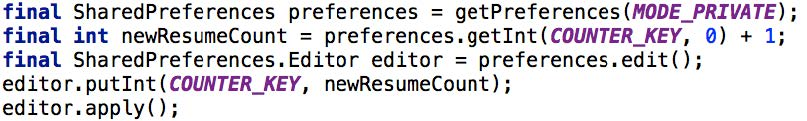
\includegraphics[width=\linewidth]{fig/preferences}
\caption{Preferences}
\label{fig:preferences}
\end{figure}

Die aus den Android Einstellungen bekannte Darstellung kann in der eigenen App auch verwendet werden. Die Einstellungen werden über eine XML-Datei (z.B. \texttt{res/xml/preferences.xml}) deklariert und mit Hilfe von \texttt{PreferenceFragement} dargestellt. \texttt{PreferenceFragment} verwendet per Default die Default Shared Preferences (1 x pro App). Abbildung \ref{fig:preference-fragment} zeigt die Erzeugung eines \texttt{PreferenceFragement}.
\begin{figure}
	\centering
	\begin{subfigure}[b]{0.48\textwidth}
		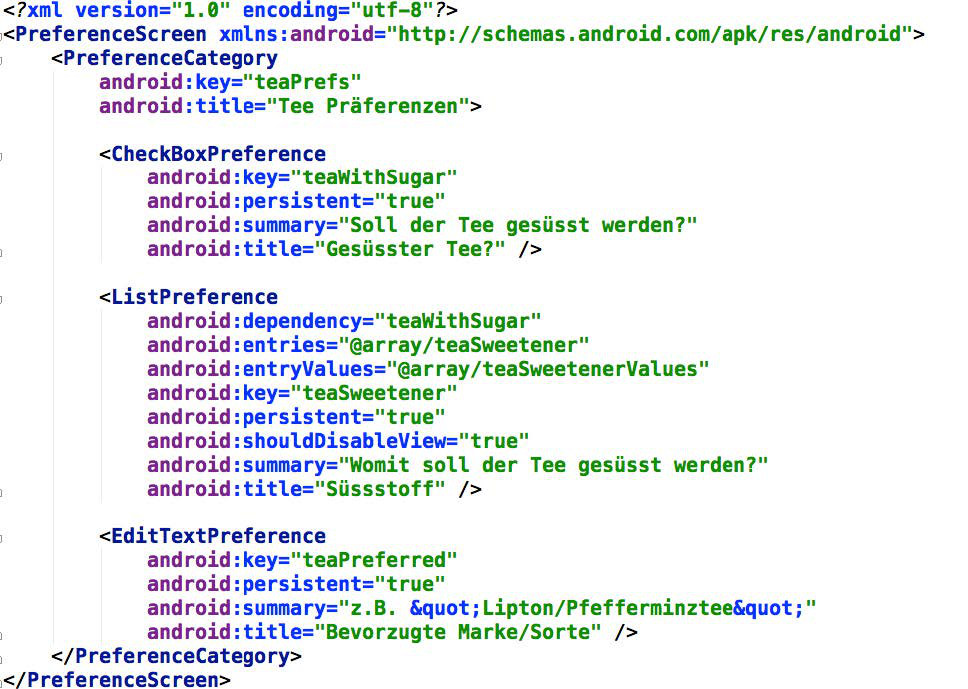
\includegraphics[width=\textwidth]{fig/preference-fragment-xml}
		\caption{\texttt{preferences.xml}}
	\end{subfigure}
	~
	\begin{subfigure}[b]{0.48\textwidth}
		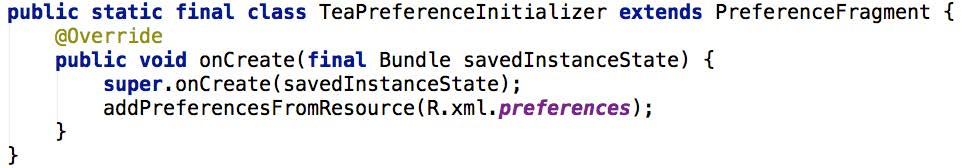
\includegraphics[width=\textwidth]{fig/preference-fragment-static}
		\caption{Statische Klasse}
	\end{subfigure}
	~
	\begin{subfigure}[b]{0.48\textwidth}
		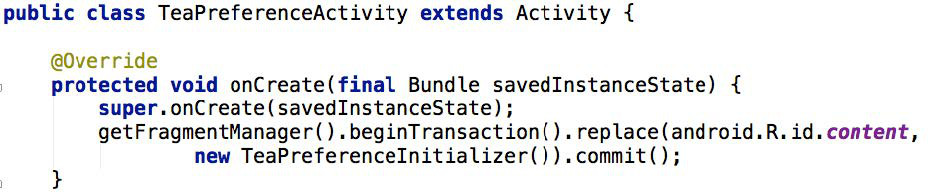
\includegraphics[width=\textwidth]{fig/preference-fragment-activity}
		\caption{Inhalt setzen}
	\end{subfigure}
	\caption{Intents aufrufen}
	\label{fig:preference-fragment}
\end{figure}

\section{Dateisystem (intern + extern)}

Dateien können entweder privat oder öffentlich sein. Private Dateien werden ins Applikationsverzeichnis abgelegt (\texttt{Context.getFilesDir()}) und andere Apps haben nur über Content Provider Zugriff darauf. Öffentliche Dateien werden auf die SD-Karte abgelegt \\ (\texttt{Environment.getExternalStorageDirectory()}). Der Zugriff auf die SD-Karte brauch eine Berechtigung im Manifest.
Für die Dateimanipulation werden die bekannten Java-Streams verwendet:
\begin{description}
	\item[Byte Datenstrom:] Für primitive Datentypen (\texttt{FileOutputStream}, \texttt{FileInputStream})
	\item[Zeichenstrom:] Für Text (\texttt{FileReader}, \texttt{FileWriter})
\end{description}
Abbildung \ref{fig:file-writer} zeigt wie in eine Datei geschrieben wird.
\begin{figure}
\centering
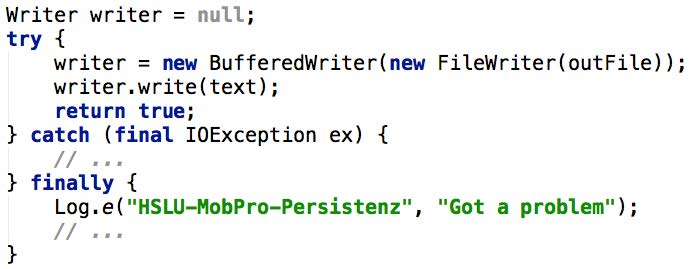
\includegraphics[width=0.7\linewidth]{fig/file-writer}
\caption{File Writer}
\label{fig:file-writer}
\end{figure}

\section{Datenbank SQLite}

SQLite ist in das Android Stack integriert und wird out-of-the-box mitgeliefert. Es wird pro Applikation eine Datenbank verwendet und andere Applikationen kriegen nur Zugriff über einen Content Provider. Android liefert kein ORM mit, sondern nur ein paar Helper-Klassen welche erweitert werden müssen. Abbildung \ref{fig:sqlite-uebersicht} zeigt eine Übersicht über sämtliche Klassen.
\begin{figure}
\centering
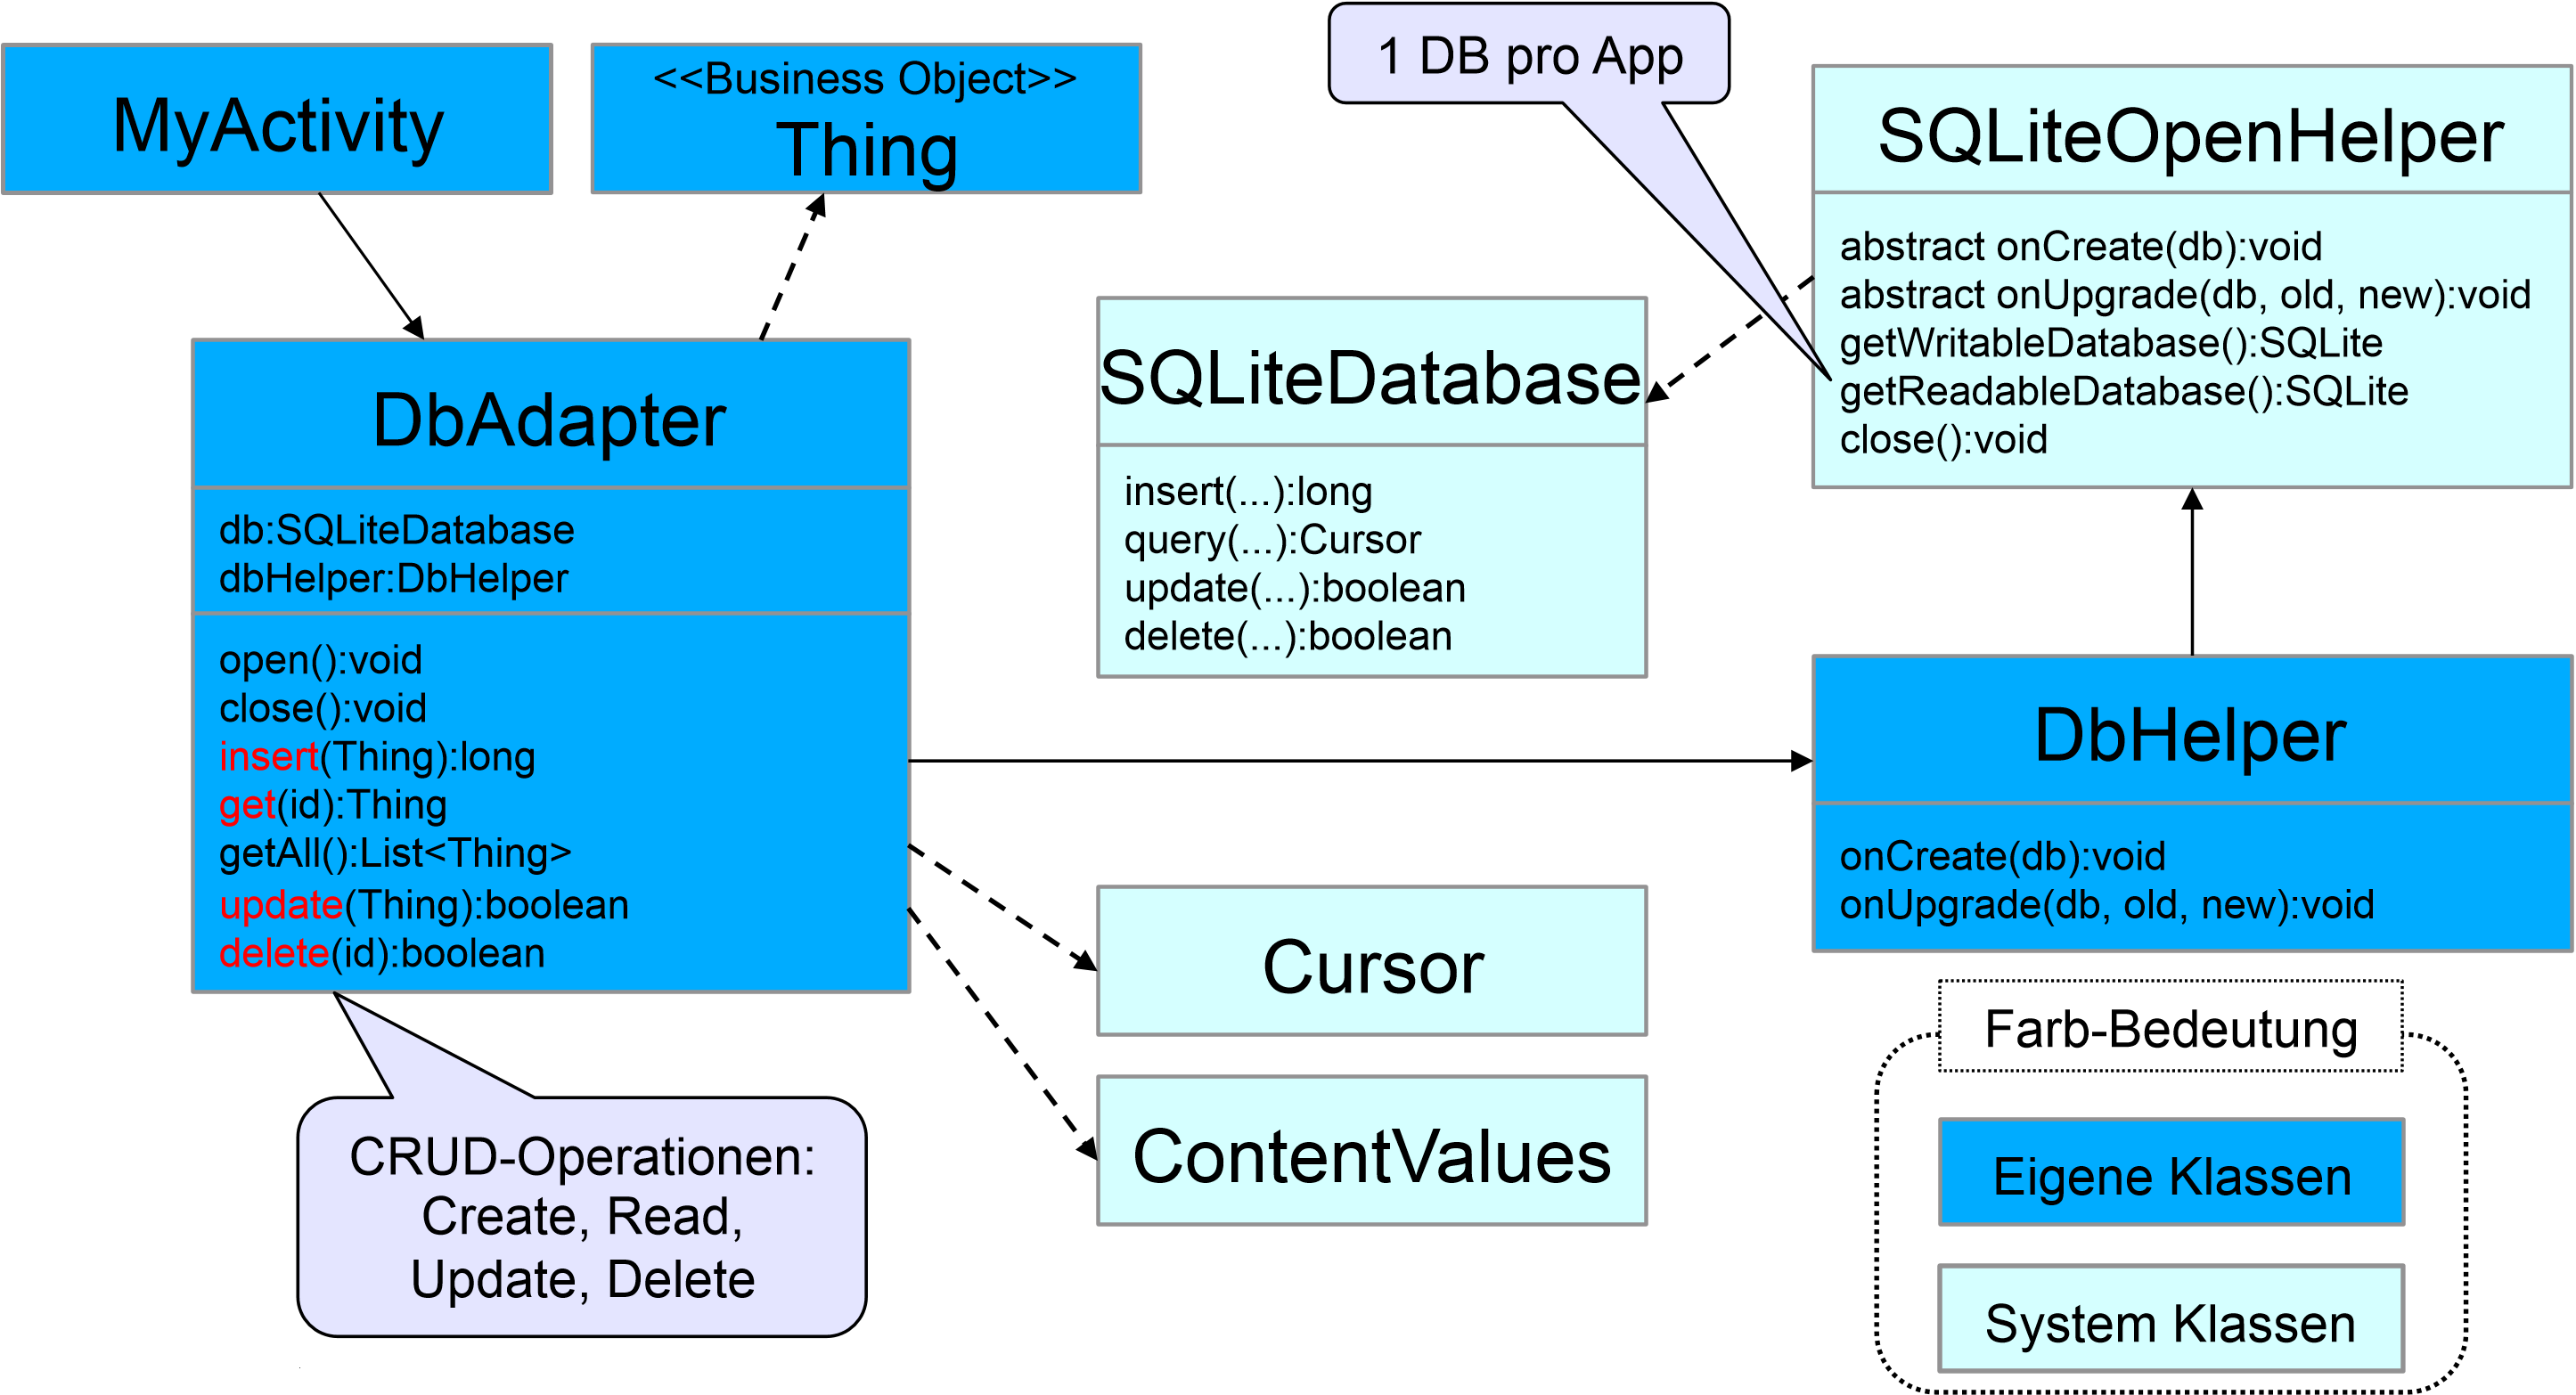
\includegraphics[width=0.9\linewidth]{fig/sqlite-uebersicht}
\caption{SQLite Übersicht}
\label{fig:sqlite-uebersicht}
\end{figure}
Eine Activity greift über den \texttt{DbAdapter} auf die Datenbank zu (Öffnen der DB in \texttt{onResume()}, Schliessen der DB in \texttt{onPause()}). Der \texttt{DbAdapter} kapselt die SQL-Aufrufe und bietet die CRUD-Operationen für die Business-Objekte an. Der \texttt{DbAdapter} benutzt den \texttt{DbHelper} um die DB zu öffnen, zu schliessen, zu erzeugen (\texttt{onCreate(db)} erzeugt Schema) und zu upgraden (\texttt{onUpgrade(db, old, new)} upgraded Schema). Abbildung \ref{fig:db-adaper-helper} zeigt eine mögliche Implementierung der oben erwähnten Klassen.
\begin{figure}
	\centering
	\begin{subfigure}[b]{0.48\textwidth}
		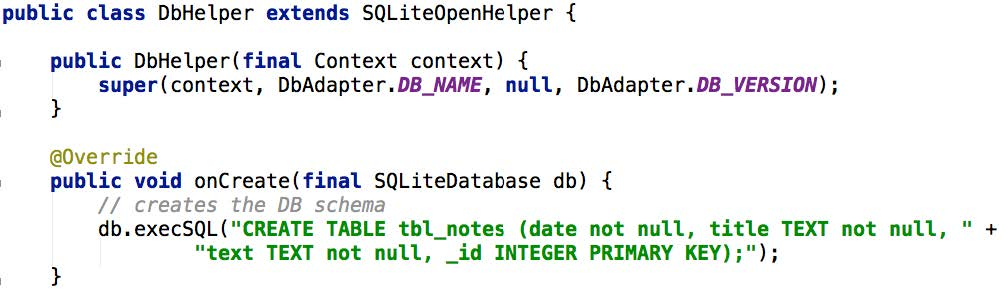
\includegraphics[width=\textwidth]{fig/dbhelper}
		\caption{\texttt{DbHelper}}
	\end{subfigure}
	~
	\begin{subfigure}[b]{0.48\textwidth}
		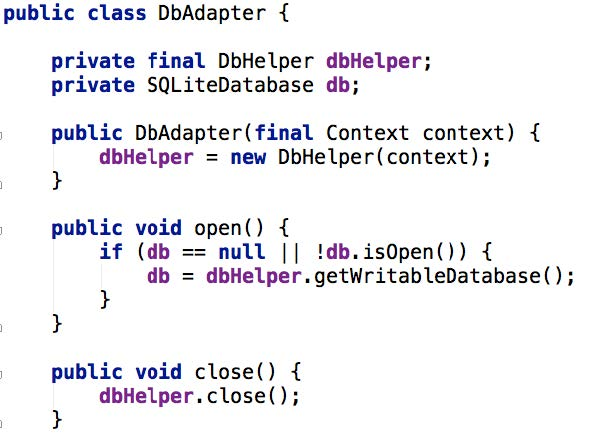
\includegraphics[width=\textwidth]{fig/dbadapter}
		\caption{\texttt{DbAdapter}}
	\end{subfigure}
	~
	\begin{subfigure}[b]{0.48\textwidth}
		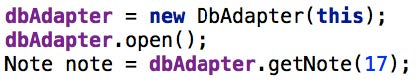
\includegraphics[width=\textwidth]{fig/dbadapter-activity}
		\caption{Aufruf in Activity}
	\end{subfigure}
	\caption{Datenbankzugriff}
	\label{fig:db-adaper-helper}
\end{figure}
Abbildung \ref{fig:crud-operationen} zeigt wie die CRUD-Operationen in einer Activity aufgerufen werden.
\begin{figure}
	\centering
	\begin{subfigure}[b]{0.48\textwidth}
		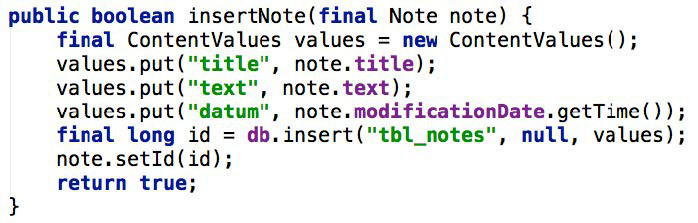
\includegraphics[width=\textwidth]{fig/sqlite-create}
		\caption{Create}
	\end{subfigure}
	~
	\begin{subfigure}[b]{0.48\textwidth}
		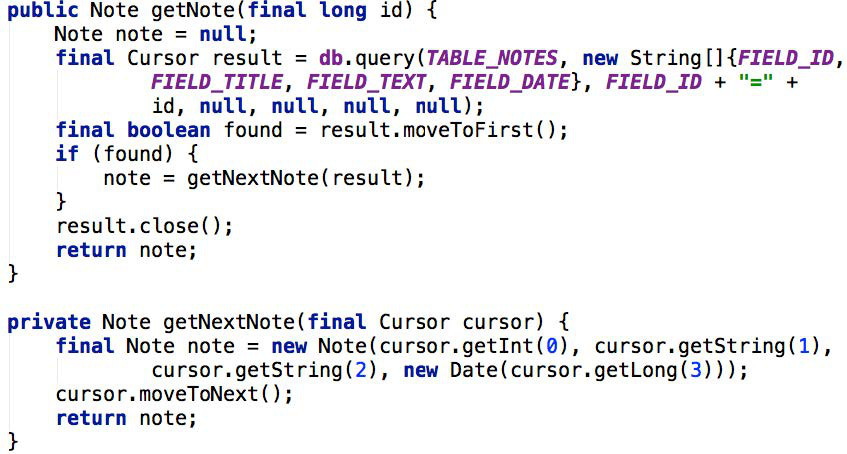
\includegraphics[width=\textwidth]{fig/sqlite-read}
		\caption{Read}
	\end{subfigure}
	~
	\begin{subfigure}[b]{0.48\textwidth}
		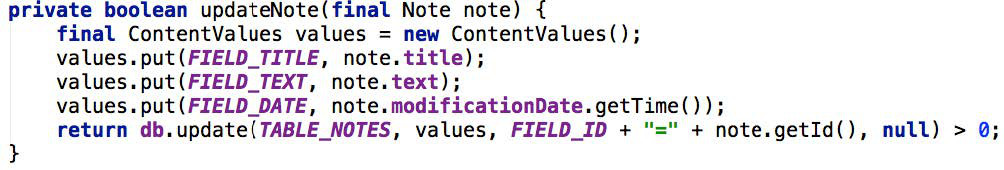
\includegraphics[width=\textwidth]{fig/sqlite-update}
		\caption{Update}
	\end{subfigure}
	~
	\begin{subfigure}[b]{0.48\textwidth}
		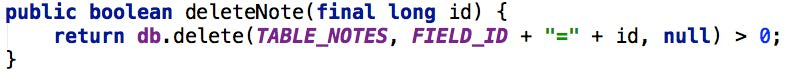
\includegraphics[width=\textwidth]{fig/sqlite-delete}
		\caption{Delete}
	\end{subfigure}
	\caption{CRUD-Operationen}
	\label{fig:crud-operationen}
\end{figure}
Das Resultat einer Query ist immer ein \texttt{Cursor}. Ein \texttt{Cursor} kann durch Resultatmenge navigieren und steht zu Beginn vor dem ersten Datensatz. Mittels \texttt{SimpleCursorAdapter} können die Daten eines Cursors relativ einfach an eine \texttt{ListView} gebunden werden (Abbildung \ref{fig:simple-cursor-adapter}).
\begin{figure}
\centering
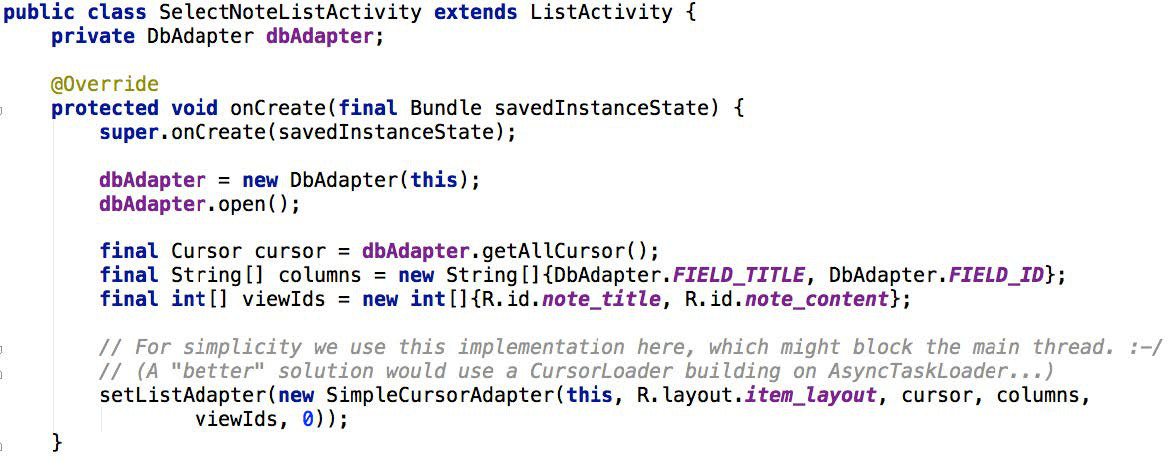
\includegraphics[width=\linewidth]{fig/simple-cursor-adapter}
\caption{SimpleCursorAdapter}
\label{fig:simple-cursor-adapter}
\end{figure}

\section{Content Providers}

Content Provider stellen für andere Applikationen Daten bereit. Daten stammen aus einer gekapselten DB oder aus dem privaten Dateisystem oder werden on-the-fly erzeugt. Der Zugriff auf die Daten erfolgt immer über eine URI (z.B. \texttt{content://<Gloable ID (FQN)>/<Welche Daten?>/ \allowbreak <Datensatz?>}). Mittels URI kann entweder ein Pfad (Datenmenge) oder ein Item (einzelnes Datenelement) angesprochen werden. Im Android-System gibt es bereits einige Content Providers, die benutzt werden können (z.B Kontakte, Browser usw.). Der Zugriff auf einen Content Provider erfolgt über einen Content Resolver (\texttt{Context.getContentResolver()}). Der Content Resolver bietet DB-Methoden (CRUD) und Zugriff auf den Content via Stream (o\texttt{penInputStream(uri)}, \texttt{openOutputStream(uri)}). Um auf gewissen Content (z.B. Kalender) zuzugreifen muss eine Berechtigung im Manifest gesetzt werden. Abbildung \ref{fig:content-resolver} zeigt wie über den Content Resolver mittels Query auf die Daten zugegriffen werden kann. Die API der Standard Content Provider ist meist schlecht dokumentiert (URI?, Projection usw.). 

\begin{figure}
\centering
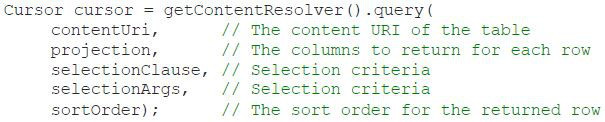
\includegraphics[width=0.7\linewidth]{fig/content-resolver}
\caption{Content Resolver}
\label{fig:content-resolver}
\end{figure}

Um einen eigenen Content Provider zu schreiben muss man von der abstrakten Klasse \texttt{android. \allowbreak content.ContentProvider} ableiten. Der Content Provider wird mit der Anwendung gestartet kann aber auch ohne laufende App genutzt werden (Start on demand). Abbildung \ref{fig:own-content-provider} zeigt welche Methoden der abstrakten Klasse implementiert werden müssen (müssen nicht alle z.B. read-only) und wie ein Content Provider im Manifest registriert wird. Einstiegspunkte (=akzeptierte URIs), Datentypen, akzeptierte Feldnamen für DB-Methoden usw. sollten in der API dokumentiert werden. Durch Setzen des Attributes \texttt{android:exported=false} ist ein Content Provider nur privat (App-intern) nutzbar.

\begin{figure}
	\centering
	\begin{subfigure}[b]{0.48\textwidth}
		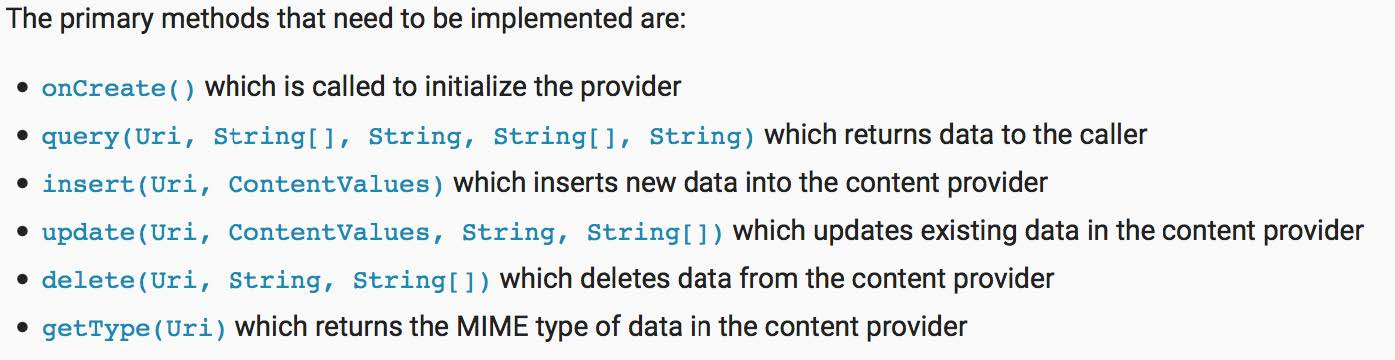
\includegraphics[width=\textwidth]{fig/content-provider-methods}
		\caption{Content Provider Methoden}
	\end{subfigure}
	~
	\begin{subfigure}[b]{0.48\textwidth}
		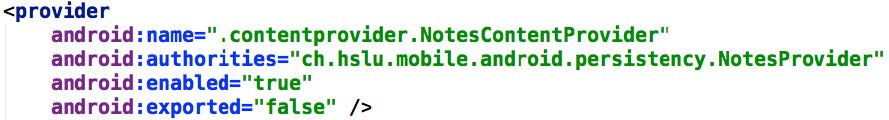
\includegraphics[width=\textwidth]{fig/content-provider-manifest}
		\caption{Content Provider Manifest}
	\end{subfigure}
	\caption{Eigener Content Provider}
	\label{fig:own-content-provider}
\end{figure}
